\section{Theoretische Grundlagen}
\subsection{Zeemann-Effekt}
Beim Zeemann-Effekt wird die Aufspaltung der Energieniveaus in Atomen durch Anlegen eines Magnetfeldes beobachtet. In unserem Experiment beobachten wir Übergänge von Elektronen im Cadmium-Atom. Die für uns wichtige Größe ist dabei der Gesamtdrehimpuls, der sich aus Bahndrehimpuls und Spin zusammensetzt, $\vec{J}=\vec{L}+\vec{S}$. Einen Zustand mit Drehimpulsquantenzahl $l$ (notiert als S,P,D,...), Spinquantenzahl $s$ und Gesamtdrehimpulsquantenzahl $j$ schreiben wir mit der spektroskopischen Notation als
\begin{align*}
  ^{2s+1}l_j.
\end{align*}
Das Atom soll sich nun in einem homogenen Magnetfeld $B$ entlang der $z$-Achse befinden (Quantisierungsachse). Dadurch wird die vorherige Entartung der Energieniveaus in der $J_z$ Quantenzahl $m_j$ aufgehoben (siehe Abb. \ref{fig:level}). In Abhängigkeit der alten Energie $E_0$ ist die neue Energie dann
\begin{align*}
  E=E_0-\frac{\mu_B}{\hbar}\left( m_j+2m_s\right).
\end{align*}
In diesem Experiment werden Übergänge 
\begin{align*}
  ^1P_1 \ \rightarrow \ ^1D_2
\end{align*}
untersucht, es gilt also $m_s=0$. Dies entspricht dem Übergang eines Valenzelektrons. Die Übergänge können durch die Änderung der Quantenzahl $m_j$ für den Gesamtdrehimpuls entlang der Quantisierungsachse charaktersiert werden. In erster Ordnung sind nur Übergänge mit $\Delta m_j=0, \ 1, \ -1$ erlaubt, die Polarisation des ausgesandten Lichtes ist dabei jeweils $\pi$, $\sigma ^+$ und $\sigma^-$.

\begin{figure}[h]
  \centering
  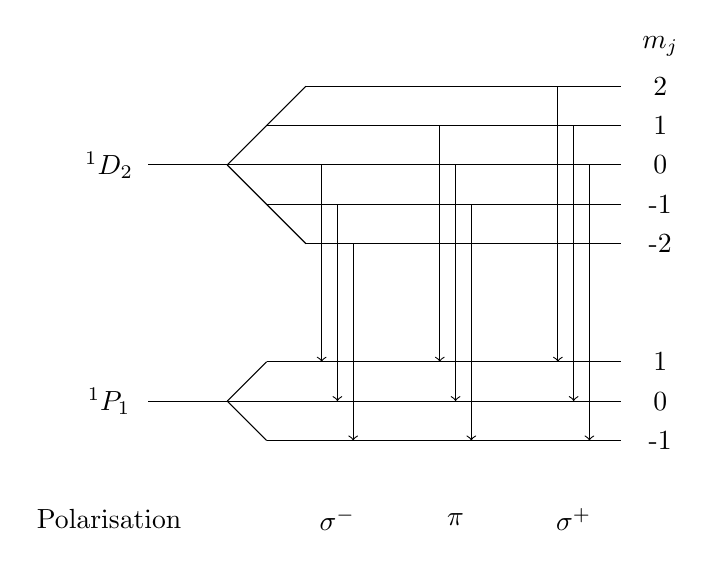
\begin{tikzpicture}
    \draw (0,0)--(6,0);
    \draw (1,0)--(2,1);
    \draw (1,0)--(2,-1);
    \draw (1.5,0.5)--(6,0.5);
    \draw (2,1)--(6,1);
    \draw (1.5,-0.5)--(6,-0.5);
    \draw (2,-1)--(6,-1);
    \draw (-0.5,0) node {$^1D_2$};
    \draw (6.5,1.5) node {$m_j$};
    \draw (6.5,1) node {2};
    \draw (6.5,0.5) node {1};
    \draw (6.5,0) node {0};
    \draw (6.5,-0.5) node {-1};
    \draw (6.5,-1) node {-2};

    \draw (0,-3)--(6,-3);
    \draw (1,-3)--(1.5,-2.5);
    \draw (1,-3)--(1.5,-3.5);
    \draw (1.5,-2.5)--(6,-2.5);
    \draw (1.5,-3.5)--(6,-3.5);
    \draw (-0.5,-3) node {$^1P_1$};
    \draw (6.5,-2.5) node {1};
    \draw (6.5,-3) node {0};
    \draw (6.5,-3.5) node {-1};

    \draw[->] (2.2,0)--(2.2,-2.5);
    \draw[->] (2.4,-0.5)--(2.4,-3);
    \draw[->] (2.6,-1)--(2.6,-3.5);

    \draw[->] (3.7,0.5)--(3.7,-2.5);
    \draw[->] (3.9,0)--(3.9,-3);
    \draw[->] (4.1,-0.5)--(4.1,-3.5);

    \draw[->] (5.2,1)--(5.2,-2.5);
    \draw[->] (5.4,0.5)--(5.4,-3);
    \draw[->] (5.6,0)--(5.6,-3.5);
    
    \draw (-0.5,-4.5) node {Polarisation};
    \draw (2.4,-4.5) node {$\sigma^-$};
    \draw (3.9,-4.5) node {$\pi$};
    \draw (5.4,-4.5) node {$\sigma^+$};
  \end{tikzpicture}
  \caption{Ausgewählte Übergänge in Cadmium}
  \label{fig:level}
\end{figure}  

Bei den betrachteten Übergängen ändert sich die Energie des $\pi$-polarisierten Lichtes also nicht mit dem Magnetfeld (wegen $m_s=0$). Bei dem $\sigma^{\pm}$ Übergängen ändert sich mit dem Magnetfeld die Energie der Photonen um
\begin{align*}
  \Delta E=\mp \mu_B B.
\end{align*}
